\chapter{Concluding remarks}\label{ch:conclusion}

\setlength{\epigraphwidth}{0.49\textwidth}%0.57
    \setlength{\epigraphrule}{0pt}%0.1
    \epigraphhead[5]{%
    \epigraph{\emph{Has been done. Can be done. Must be done\ldots}}%
    {Fandarel \mycite{McCaffrey}}
}

With the recent profusion of expression atlases
and the steadily growing number of independent studies
integrating these atlases' data as-is\footnote{%
More than 2,800 citations on 15 September 2019 for five human studies},
it has become increasingly imperative to examine
the soundness of their extensive use in unrelated research.

At the time I started my doctorate,
no assessment on the robustness of expression or
comparison between independent \Rnaseq\ datasets was published yet.
Thus,
my primary aim was to integrate and compare independent transcriptomic data
as they were the only available human tissue data.
However, the release of two substantial proteomic datasets in the meantime
broadened my study's scope
to the additional integration of transcriptomic with proteomic data.

In \Cref{ch:background},
I reviewed the biological, chemical and bioinformatic aspects and challenges
involved in expression studies based on the high-throughput technologies
of \Rnaseq\ (for \mRNAs) and \ms{} (for proteins).

Then in \Cref{ch:datasets},
I presented the five transcriptomic and three proteomics studies
that I have considered for this thesis.
I also described the pipelines with which I have processed them.
Since for each dataset the number and size of files are extremely important,
automation is paramount to ensure consistency and minimise errors.\mybr\

I detailed in \Cref{ch:expression} various data quality controls
and statistical approaches.
I also discussed possible biases and
how the contextual scope of the tissues and genes considered for analyses
can influence results.
To minimise errors due to context issues,
I limited most of my further investigations to
a common subset of tissues and expressed genes.
Normalisation methods are still inadequate
to treat mitochondria genes accurately.
Therefore, I chose to remove them from most analyses,
which led to better results.

In \Cref{ch:Transcriptomics},
I integrated the five independent transcriptomic datasets and
showed that the biological signal is predominant to the technical noise.
All datasets have a higher interstudy correlation for the same tissues
than any intrastudy correlation for different tissues.
The more recent the studies are, the stronger this trend is.
I then tested various criteria as possible driving forces
of the high interstudy correlation.
I found that most variable genes and Tissue-Specific (\gls{TS}) genes
are individually contributing more to the high correlations
than the highest expressed ones.
Besides, I also noted that
the inclusion of external resources requires caution,
especially when the resources are outdated, such as \gls{TIGER}~\mycite{tiger}.
Many \gls{TS} genes highlighted by \Rnaseq\ are missing in this database.
Besides, many listed genes are either wrongly attributed to another tissue
or lack to display any specificity.
The integration has revealed that
direct comparisons of independent data may be impossible yet,
but genes present identical overall profiles across the studies.
By repeatedly showing this similarity, my analyses prompted
the creation of the heatmap visualising expression data
(and its associated widget) for baseline expression data in
\hFoCi{Expression Atlas}{https://www.ebi.ac.uk/gxa/home}{EBIgxa}.
Finally, I provide a core set of genes that are expressed consistently
(ubiquitously or \gls{TS}) across all studies.\mybr\

The comparison of three available proteomic datasets
in \Cref{ch:proteomics} highlights
the fragmentation and the disparity of the high-throughput \ms{}-based proteomics.
\ms\ detection variability induces considerable technological noise,
which explains
the intrastudy correlations I observed between different tissues are
higher than the interstudy correlation for the same tissues.
I provide curated sets of the \gls{TS} and ubiquitous detected proteins.
Finally, I present a new quantification method that
I have devised by drawing on \Rnaseq\ methods.
By also accounting for \emph{degenerated} peptides,
this \PPKM\ method allows us to quantify more proteins.\mybr\
%\mybr\
%These latter are distributed according to the distribution of \emph{unique} peptides
%between the possible parent proteins.

\Cref{ch:Integration} reported
the integration of the independent proteomic and transcriptomic data.
For these independent studies,
I have found correlation levels
(Spearman correlation $0.39 ≤ \rho\ ≤ 0.62$)
similar to the ones typically observed in
the literature for same-sourced proteome and transcriptome.
The \PPKM\ quantification improves the Pearson correlation
and gives similar ranges to Spearman ($0.38 ≤ r ≤ 0.61$).
Two tissues exhibit distinct characteristics across the various analyses
(and literature): \Testis\ and \Liver.
\Testis\ has the most diverse and specific expression
at both transcriptomic and proteomic levels.
On the other hand, \Liver\ has the most robust expression across studies
and the highest correlation between its \mRNAs\ and proteins expression levels.
Overall, the tissues feature mixed correlation levels,
and it is impossible to predict protein expression from \mRNA{}.
However, there are shared coherent gene signatures
between the proteome and transcriptome
that are even detectable through indirect analyses for a few.
Furthermore, once again,
\mRNAs{}' and proteins' tissue specificity is contributing
more to the tissue correlation than their expression levels.
In addition to the significant overlaps of \gls{TS} proteins
with the most \gls{TS} \mRNAs,
most pairs comprising a \gls{TS} protein have
a high correlation between their RNA and protein expression across tissues.
Finally, \gls{go} analyses show that \enquote{pairs with a \gls{TS} protein}
are enriched for specific signalling,
including its detection, response pathway and regulation.
The \enquote{highest correlated pairs} are
enriched for catabolic processes.
Lastly, the \enquote{most anticorrelated pairs} show enrichment
for ribosome complexes and \glspl{ncRNA} regulation.
I provide the complete set of \mRNA/protein pairs with their correlation
across the common set of tissues.
I also supply the list of overlapping \gls{TS} proteins and \mRNAs{}.\mybr\

I provide the necessary code to replicate all of the above results (and more)
as \href{https://github.com/barzine/BaselineAtlas/tree/thesis.}{supplementary
material}\footnote{\Href{https://github.com/barzine/BaselineAtlas/tree/thesis}}.


Throughout this thesis' analyses,
I had to overcome many practical challenges.
While most of the difficulties encountered ordinarily pertain to Big data projects,
one unexpected issue was
the current global complexity state of the proteomic world.
Physicochemical properties of the proteins make them
intrinsically complex to study,
as shown in \Cref{sec:exploreProtMS}.
The characterisation of proteins (or assimilated complexes) represents
a technical obstacle for many different fields
(\eg\ molecular biology, medicine, drug design, green chemistry),
which may explain the transposition of the technical complexity
to the conceptual level.
Understand high-throughput proteomics requires many prerequisites,
and because of the many possible approaches,
the available teaching materials are mostly
practical or experimental oriented~\mycite{Zhang2013,Zhang2014,LCMSconsider} or
on particular steps, \eg\ protein inference~\mycite{He2016-yi}.
The scattered information hampers the ability of newcomers
to achieve a global vision of high-throughput proteomics easily.\mybr\

Big data is often characterised through, what was first defined by
\href{https://www.ibm.com}{IBM}\footnote{\Href{https://www.ibm.com}},
the \emph{4 V's}: volume, variety, veracity and velocity.
Each of them can entail issues at different project levels.

The volume of files (see \Cref{tab:Lib5DF})
to handle and process just for the transcriptomics
is overwhelming and requires properly dimensioned infrastructure
like in the \gls{EBI}.
It is in practice impossible to reproduce the complete work underlying
this thesis in a personal computer within a reasonable time.
Although (commercial) solutions are increasingly in use for academic projects,
dedicated storage and high computing facilities ease the analyses considerably
and allow more in-depth testing.
Even if best practices are continuously refined for transcriptomics,
there are still many factors that can be improved and tuned.
So, besides the raw data,
storage capacity is also required for the intermediate and final ones.
Also, organising such a large amount of data was challenging at times.

The variety of the input data is kept to a minimum for the expression value
as it was retrieved from public or academic repositories
that follow community guidelines\footnote{%
\href{https://www.ebi.ac.uk/ena}{ENA} for the sequencing data and
\href{http://www.proteomexchange.org}{ProteomeXchange} for \ms/\ms/ proteomics.
}.
Issues still ensue from the matchmaking
between the samples or tissues across the studies.
For many tissues, I chose to mix several \enquote{body parts}
(from the same tissue though) in \gtex\
to match them to the other studies' tissues.
Perhaps, in some case, one \enquote{body part} is perfectly matched
to the samples from another study
where the authors have only reported the tissue instead.
Hence, for these cases,
keeping only one of the \enquote{body parts}
would have been a better choice.

Another source of variety that I have limited in the above work
is the diverse annotation versions.
Even when mapped to the same genome and annotation versions,
discrepancies persist between how transcriptomics and proteomics
are defined and assigned to the genes.
A possible improvement of the present work will be to use
the chromosome coordinates to which \mRNAs\ and proteins map
instead of using their gene identifiers (\gls{Ensembl} ID).\mybr\

Additionally, with all possible tunable parameters for the raw data processing,
the generated data to integrate can vary quickly.
Even with a limited number of combinations,
my study shows that the results' trend remains the same
regardless of the chosen settings.
Moreover, as the number of datasets I included in my analyses grows,
the results became increasingly stabler.
Many of them have also been confirmed by the literature,
adding credibility and confidence to the findings,
especially considering the recent discussions on reproducibility crisis~\mycite{%
Morrison2014-hy,Glenn_Begley2015-fz,Goodman2016-ri,Fatovich2017-lo,
Coiera2018-vf,Lindner2018-qy}.
However, results for individual genes can vary from one set of settings to another one,
and need to be considered with more caution.

Finally, the velocity of new data availability
and its required preparation time
before possible inclusion in my on-going analyses
made the prospect impracticable.
Unfortunately, although new \gtex\ samples or other tissues studies
(\eg\ Oncobox Atlas of Normal Tissue Expression (ANTE)~\mycite{Suntsova2019-it})
kept being released,
I had to stop including them in my study.
Likewise, I ceased updating the genome and annotation
and settled for \hg{38.p1} and \ens{76}.

To minimise errors,
assure consistency and ease future reiterations or extension of these analyses,
I provide script files that can reproduce the whole study and its results.
I have also automated and structured the analyses through modular functions
as much as possible.
It is important to avoid undocumented manual changes,
so even name changes and sample pairings are done through scripts.\mybr\

I chose to develop the analyses with open-source software
around the programming language \WebFoCi{\textsf{R}}{https://cran.r-project.org}{coreR}.
See \Cref{sec:Rpackages} for the complete list of \textsf{R} packages
involved in this work.
This language provides statistical and visualisation functions
and is easily expanded through packages developed by the community.
Packages can be highly interdependent and may evolve rapidly.
To draw from an extra package (or fix an identified bug),
a comprehensive and time-consuming update of the working environment
will often ensue.
In turns, I had also to update my analyses' code in many occasions.
Furthermore, new software installations or updates are more complicated
for distributed computing facilities than on a personal computer.
Today, new solutions are developed to facilitate these tasks
(\eg\ \softCi{Packrat}{Rpackrat} that create isolated environment).

Note that \nuno, who provided me with the quantification of the \gtex\ data,
and \james, who provided me with the proteomics ones,
have also both developed their processing pipelines with open source software.
Hence, the entirety of the thesis (subject to access to \gtex\ data)
can be repeated easily.\mybr\

If that were the case, many improvements are conceivable:
\vspace{-3mm}
\begin{itemize}[topsep=0pt,nosep]
        \item The inclusion of new samples and dataset of transcriptomics
            (preferably with biological replicates),
            \eg\ extend to the last version of \gtex\ and
            the ANTE dataset~\mycite{Suntsova2019-it}.
        \item Add the matching proteomics of \citet{Wang2019-ut}
            to the transcriptomic \uhlen\ data~\mycite{Uhlen2015}
            and then compare the results to the unmatched samples.
        \item Work on new models of annotation or
            build a consensus between the current transcriptomic and proteomic
            annotations.
            Today, it is difficult to determine for some genes
            (\eg\ \gene{STAU2})
            if the observed anticorrelation or lack of correlation
            between the \mRNA\ and protein expression levels is due to the biology,
            batch effects or divergences between transcriptomic and
            proteomic annotations.
        \item Changing the quantification (parameters or methods)
            may also give better results.
\end{itemize}
%The potential for improvement due to quantification is appealing.\mybr\

Most normalised quantification methods are designed
for differential expression studies,
particularly in transcriptomics.
As a result, they are ill-suited
for comparing independent samples across multiple studies.
However, two other normalisation methods
do not imply any preconception on the study design.
\gls{FPKM}~\mycite{Mortazavi2008,cufflinks},
which I use in this thesis,
and TPM (Transcript per Million)~\mycite{Wagner2012-du}.
Both normalisation methods account for the global library size of each sample.
While the motivation is sound\footnote{For \FPKM, see \Cref{subsub:norm}.
\FPKM\ is easily converted to TPM by scaling with a constant
to correct the sum of all values in a library to 1 million.
},
the quantification is thus contextual
to %which
how many
and how much \glspl{RNA} are detected.
Previous efforts to solve this problem have focused
on differential expression studies.
Synthetic spike-in molecules~\mycite{Jiang2011-ux}
ensure more reliable quality controls.
However, they fail to permit the absolute quantification
of the other molecules in the sample.
Incidentally, \citet{Rudnick2014-ar} find that spike-in proteins and peptides
lack effectiveness for proteomic studies.
For proteomics, \citet{Wisniewski2014-kh} propose
to use the histone to create a \enquote{\emph{proteomic ruler}}.
They can assess through this proteomic ruler the amount of \gls{DNA}
in the sample, and thus, giving an estimate on the cell number,
which provides some context to interpret the quantification of the proteins.
Histone genes are, however, ill-suited
for bulk \Rnaseq\ studies~\mycite{Zhao2018-rw}.

I firmly believe that using internal standards chosen
within the naturally expressed population of the studied macromolecules
is more appropriate than any external additive.

Gene length (and possibly other biases)
has to be accounted for an appropriate normalisation of expression.
However, I expect that normalising the expression of each gene (RNA or protein)
as a rational expression to a reference gene will be more robust
than normalising for the library size as a means to correct
for the sequencing (or coverage) depth between samples size.
A ratio will free the expression of any influence
from the presence or quantification of any other gene.
Then, the next question is:
\enquote{Which gene (or set of genes) will possibly enable the best normalisation?}

Through this thesis' various analyses,
I have highlighted genes that have a robust and ubiquitous expression
across all the studied tissues
both at transcriptomic and proteomic levels.
Moreover, many genes present high correlation coefficients
between the expression of their \mRNA\ and protein.
These genes are the best potential candidates as reference.
With \nuno, we have performed preliminary analyses
in this direction across other studies
to reduce the list of these candidates.

However,
considering the best practices in analytical chemistry~\mycite{analyticalChem},
a set of standards that can cover the complete dynamic ranges of abundances
and adjust for the saturation effects,
may resolve the abundances better,
and thus, be better suited than a single reference.
On the other hand, studies focusing on a single tissue
may better benefit from a reference built on \gls{TS} genes.

The recent development of single-cell transcriptomics
(scRNA-Seq)~\mycite{Chen2019-um},
and the probable feasibility of single cells proteomics~\mycite{Marx2019-cf},
may ease refining which genes are the most suitable as universal references,
or for specific conditions.

%\vspace{-1mm}
Integrating proteomics and transcriptomics remains laborious,
and results can be mitigated.
Nonetheless,
even simple comparisons % of independent data
can help to improve our general knowledge
and current biological models.
For instance, in one of our papers % \citetitle{Wright-2016}
\mycite{Wright-2016},
we have confirmed the existence of putative proteins
by observing coverage of the genome both by transcriptomics and proteomics.

%\vspace{-1mm}
To help further possible projects,
I am currently compiling the different analyses
into a set of interactive applications
that can replicate all the results and figures presented in this thesis
without requiring any programming skill as a prerequisite.
\Cref{fig:demoApp} covers \Cref{ch:expression}.

%\vspace{-1.5mm}
\begin{figure}[!ht]
    \frame{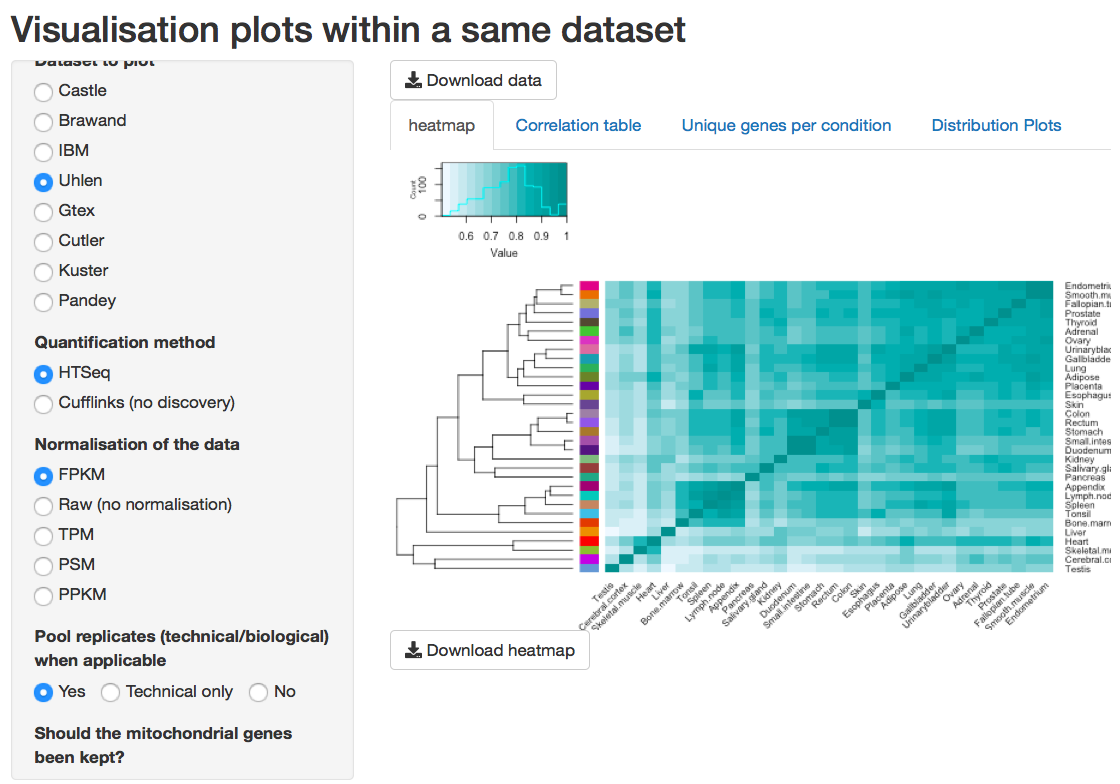
\includegraphics[scale=0.31]{conclusion/demoApp.png}}\centering
    \vspace{-2mm}
    \caption[Application preview]{\label{fig:demoApp}\textbf{Preview of the
    application} developed with \textsf{R}
    and served through a shiny~\mycite{shinyR} server.}
\end{figure}
%\vspace{-3mm}
Once completed, one will be able to analyse and compare their own data
to the different datasets I have presented in this thesis.
Furthermore, as I share all my code (including for the application)
under a creative commons license,
\WebFo{Attribution 4.0 International  (CC BY 4.0) 
\includegraphics[width=1em]{cc.pdf}%

\includegraphics[width=1em]{by.pdf}}{https://creativecommons.org/licenses/by/4.0}.
Anyone can thus use, adapt or build upon this work as they wish.


%Achievements
% Showed that mitochondrial \mRNAs\ and proteins should be excluded from the bulk
% (even though separate analysis can be considered)
%
% Transcriptomics present similar profiles: tissue across datasets,
% and \mRNAs\ profiles through the tissues across datasets.
% This finding has prompted the EBI heatmap visualisation
%
% New proteomics quantification methods inspired on transcriptomic ones
% can increase the number of quantified proteins
% while seemingly unkooky
%
% First time so many different data have been mapped to the same genome version
% and annotation with identical pipelines.
% Quite in-depth comparison between Uhlen and \gtex.
% Reprocessing of all the untarget non-diseased human proteome
%
% Consolidated gene lists for consistent transcriptomic expression
%                                           (modified Uhlen categories)
%                 and for matched (but independently sourced) \mRNA/protein pairs
%                     for TS, highly correlated and very anticorrelated
%
% Organs show constant catabolic profile (set of genes) that have
% mRNAs/proteins expression consistent through aggregation of individual and
% across different datasets.
% Particularly, housekeeping and TS genes
%
% Testis most diverse and unique expression
% Liver most robust expression
%


